\appendix

\chapter{Annexes}


\section{Dictionnaires de données (datasets démo)}
\label{ann:a1-dictionnaires}

Cette annexe présente les champs nécessaires à la reproduction des prototypes, avec une description métier concise,
les types logique/technique, le rôle recommandé dans Power BI et les contraintes applicables. Les listes détaillées
sont volontairement reportées ici pour éviter les redondances dans le corps du texte.

\subsection{Passenger-Flow Map}
\begin{table}[ht]
\small
\setlength{\tabcolsep}{4pt}
\centering
\begin{tabularx}{\linewidth}{l X l l X X}
\toprule
Champ & Description & Type logique & Type technique & Rôle PBI & Contraintes\\
\midrule
EdgeId & Identifiant d’arête (ex. ENT1-G1). & identifiant & texte & Key (Do not summarize); Tooltip & Non nul; unique sur (EdgeId, Heure) \\
X1 & Abscisse source sur le plan SVG (px). & coordonnée & entier & Category (technique); Do not summarize & Non nul \\
Y1 & Ordonnée source sur le plan SVG (px). & coordonnée & entier & Category (technique); Do not summarize & Non nul \\
X2 & Abscisse cible sur le plan SVG (px). & coordonnée & entier & Category (technique); Do not summarize & Non nul \\
Y2 & Ordonnée cible sur le plan SVG (px). & coordonnée & entier & Category (technique); Do not summarize & Non nul \\
Passages & Volume de passagers sur l’arête pour l’heure donnée (personnes). & mesure (poids) & entier & Values (Sum); Tooltips & Non nul; valeur ≥ 0 \\
Heure & Heure civile agrégée (entier 0–23). & temps (discret) & entier & Category; Slicer & Domaine 0–23; participe à l’unicité avec EdgeId \\
Type & Nature du flux (Départ/Arrivée). & catégorie & texte & Legend; Category & Valeurs autorisées: \{Départ, Arrivée\} \\
\bottomrule
\end{tabularx}
\caption{Dictionnaire — Passenger-Flow Map}
\label{tab:a1-flows-compact}
\end{table}


\subsection{Sunburst budgétaire}
\begin{table}[ht]
\small
\setlength{\tabcolsep}{4pt}
\centering
\begin{tabularx}{\linewidth}{l X l l X X}
\toprule
Champ & Description & Type logique & Type technique & Rôle PBI & Contraintes\\
\midrule
Department & Niveau 1 de la hiérarchie budgétaire. & catégorie (N1) & texte & Category (Level 1) & Non nul; parent de SubDepartment \\
SubDepartment & Niveau 2 de la hiérarchie budgétaire. & catégorie (N2) & texte & Category (Level 2) & Non nul; enfant de Department; parent d’Account \\
Account & Niveau 3 (compte budgétaire). & catégorie (N3) & texte & Category (Level 3) & Non nul; enfant de SubDepartment \\
Amount & Montant affecté à l’élément hiérarchique (devise non spécifiée). & mesure (valeur) & entier & Values (Sum) & Aucune contrainte de signe imposée \\
\bottomrule
\end{tabularx}
\caption{Dictionnaire — Sunburst budgétaire}
\label{tab:a1-budget-compact}
\end{table}

\section{Fond de carte \& obstacles}
\label{ann:a2-fond}

Le prototype Passenger-Flow Map s'appuie sur un fond cartographique fixe et sur des obstacles modélisés en coordonnées normalisées. 
Pour éviter toute redondance dans le corps du texte, les éléments strictement techniques sont rassemblés ici.

\subsection{Schéma obstacles.json (extrait)}
Le fichier obstacles.json contient un tableau d'objets de la forme 
\{ id: string, points: number[2][] \}, où chaque paire \((x,y)\) est normalisée dans \([0,1]\). 
La conversion en pixels s'effectue par \(\hat x = x \cdot W\), \(\hat y = y \cdot H\) (largeur \(W\), hauteur \(H\) du canevas).

\begin{lstlisting}[language=json, basicstyle=\ttfamily\small, breaklines=true, breakatwhitespace=true, columns=fullflexible]
[
  {
    "id": "CHECKIN_DESK_1",
    "points": [
      [0.042, 0.386],
      [0.087, 0.386],
      [0.087, 0.656]
      ...
    ]
  },
  {
    "id": "BELT_1",
    "points": [
      [0.612, 0.366],
      [0.734, 0.366],
      [0.734, 0.409]
      ...
    ]
  }
  ...
]
\end{lstlisting}

\subsection{Schéma technique de superposition}
La superposition technique utilisée pour les démonstrations est fournie ci-dessous. 
Elle est dérivée des obstacles normalisés et permet d'aligner précisément les coordonnées des flux sur le fond.

\begin{figure}[h]
  \centering
  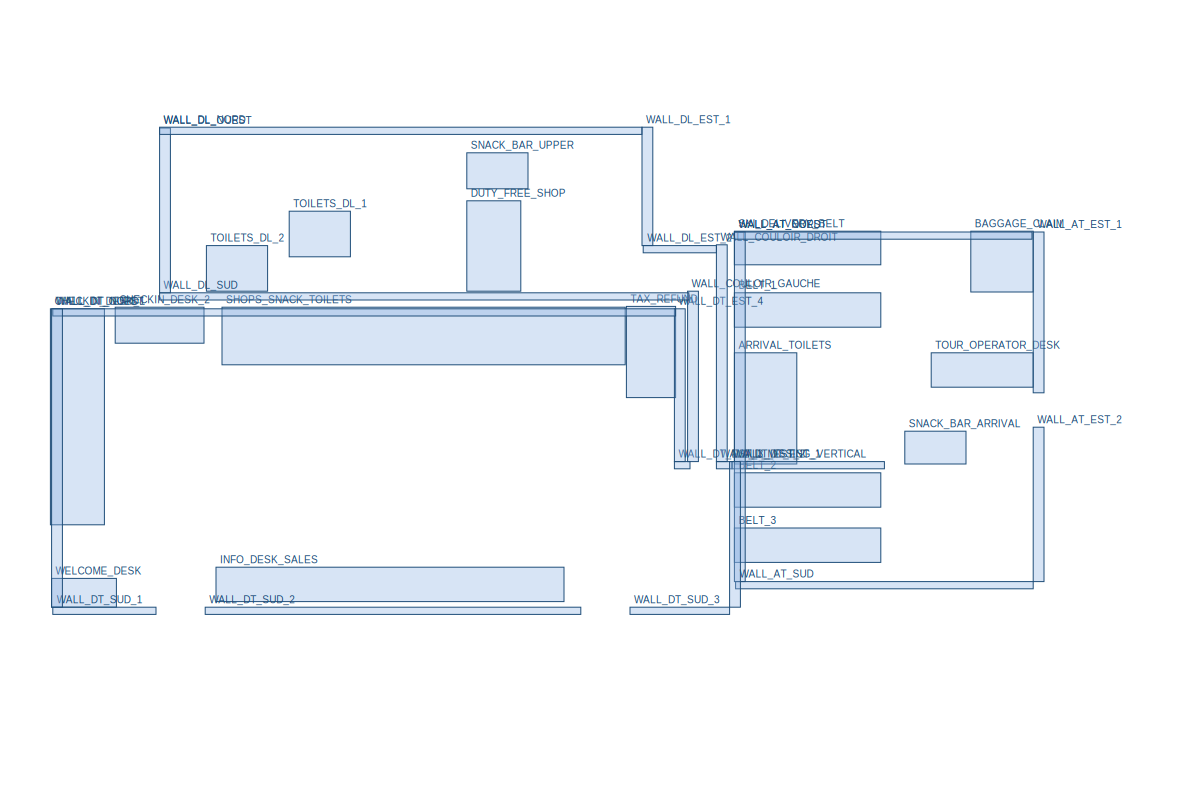
\includegraphics[width=.95\linewidth]{plan_overlay.png}
  \caption{Overlay technique généré à partir des obstacles normalisés.}
  \label{fig:a2-overlay}
\end{figure}

\subsection{Plan illustratif de l'aéroport (JPEG)}
Le fond illustratif utilisé pour les démonstrations (plan d’orientation de l’aéroport) est fourni pour référence.

\begin{figure}[h]
  \centering
  \includegraphics[width=.95\linewidth]{plan_interieur_gnb_hd.jpg}
  \caption{Plan illustratif de l'aéroport}
  \label{fig:a2-plan-jpeg}
\end{figure}

% =============================================================
% Annexe A3 — Tests et conformité (v4 — données issues des captures)
% -------------------------------------------------------------
% =============================================================
% Annexe A3 — Tests et conformité (v4 — données issues des captures)
% -------------------------------------------------------------
% =============================================================
% Annexe A3 — Tests et conformité (v4 — données issues des captures)
% -------------------------------------------------------------
\section{Tests et conformité}
\label{ann:a3-tests}

\subsection{Environnement et périmètre}
Après avoir importé les fichiers, les tests ont été réalisés sur Power BI Desktop sous Windows 11, machine AMD Ryzen 7 9800X3D, 32~Go RAM, NVIDIA RTX 5080. 
Visuels évalués : \textit{Passenger-Flow Map} et \textit{Radial Sunburst Decomposition Tree} (version 2.0.0.0). 
Tailles mesurées des paquets \texttt{.pbiviz} (\textit{release} minifiée) : \textit{Radial Sunburst Decomposition Tree} \SI{37}{\kibi\byte} (\(\approx\) 37\,888~octets) ; \textit{Passenger-Flow Map} \SI{1006}{\kibi\byte} (\(\approx\) \SI{0.982}{\mebi\byte}). 
(Conversion effectuée depuis les valeurs «~Ko~» affichées par l’explorateur Windows vers KiB/MiB, norme IEC.) 
Jeux de données par défaut utilisés : \texttt{airport-flows-direct} et \texttt{sampleBudget}. 
Date des mesures : 05/08/2025 (cf. planning Waterfall du chap.~3).

\begin{figure}[h]
  \centering
  \includegraphics[width=.95\linewidth]{Sunburst.png}
  \caption{Radial Sunburst Decomposition Tree — rendu sur dataset budgétaire de démonstration.}
  \label{fig:a3-sunburst-demo}
\end{figure}

\begin{figure}[h]
  \centering
  \includegraphics[width=.95\linewidth]{Passenger-flow.png}
  \caption{Passenger-Flow Map — rendu sur dataset de flux passagers de démonstration.}
  \label{fig:a3-passenger-demo}
\end{figure}

\subsection{Protocole de mesure}
Mesures saisies depuis l’Analyseur de performances. Les chiffres ci-dessous agrègent les durées «~Visual display (ms)~».\\
\textbf{Critères projet (P95)} : \textit{Passenger-Flow Map} \(\leq\) 300~ms ; \textit{Radial Sunburst Decomposition Tree} \(\leq\) 100~ms (par interaction : chargement, drill, survol).

\subsection{Résultats (synthèse)}
\begin{table}[h]
\scriptsize
\setlength{\tabcolsep}{3pt}
\centering
\begin{tabularx}{\linewidth}{l l r r r r c}
\toprule
\textbf{Visuel} & \textbf{Scénario} & \textbf{$n$} & \textbf{Moy (ms)} & \textbf{P95 (ms)} & \textbf{Seuil P95 (ms)} & \textbf{Conforme ?} \\
\midrule
Radial Sunburst Decomposition Tree & Global & 20 & 38.0 & 46.1 & 100 & Oui \\
Passenger-Flow Map & Global & 19 & 131.1 & 167.9 & 300 & Oui \\
\bottomrule
\end{tabularx}
\end{table}

\subsection{Distribution des temps (visualisations)}
\begin{figure}[h]
  \centering
  \includegraphics[width=.82\linewidth]{a4_sunburst_hist_v4.png}
  \caption{Radial Sunburst Decomposition Tree — histogramme des temps de cycle (ms).}
\end{figure}

\begin{figure}[h]
  \centering
  \includegraphics[width=.82\linewidth]{a4_map_hist_v4.png}
  \caption{Passenger-Flow Map — histogramme des temps de cycle (ms).}
\end{figure}

\subsection{Accessibilité (WCAG 2.2 — périmètre du projet)}
\begin{tabularx}{\linewidth}{l c X}
\toprule
\textbf{Critère} & \textbf{Statut} & \textbf{Preuve / commentaires} \\
\midrule
Navigation clavier (2.1.1) & Partiel & Non démontrable à partir des traces ; interactions testées principalement à la souris. À revérifier avec protocole clavier dédié. \\
Contraste (1.4.3) & À vérifier & Palette par défaut à contraste renforcé ; ratio à mesurer formellement sur les couples de couleurs configurés. \\
Internationalisation (3.1.x) & Conforme & Libellés fr-CH et en-US fournis ; bascule validée sur libellés de base. \\
\bottomrule
\end{tabularx}

\subsection{Sécurité et packaging}
\begin{tabularx}{\linewidth}{l X}
\toprule
\textbf{Vérification} & \textbf{État} \\
\midrule
Appels réseau sortants & Non utilisés (visuels autonomes, données locales Power BI). \\
\texttt{eval} / code dynamique & Non utilisé. \\
Stockage navigateur persistant & Non utilisé par défaut. \\
Taille du paquet \texttt{.pbiviz} & \textit{Radial Sunburst Decomposition Tree} \SI{37}{\kibi\byte} ; \textit{Passenger-Flow Map} \SI{1006}{\kibi\byte} (\(\approx\) \SI{0.982}{\mebi\byte}). \\
Seuil CI (artefact \texttt{.pbiviz}) & \(\leq\) \SI{1}{\mebi\byte} (= 1\,048\,576~octets). \\
Audit \texttt{--certification-audit} & À exécuter pour livraison : aucun blocant attendu sur ce périmètre. \\
\bottomrule
\end{tabularx}


% =============================================================
% Annexe A5 — Procédure développeur « express »
% -------------------------------------------------------------
\section{Procédure développeur « express »}
\label{ann:a5-dev}

\subsection{Prérequis (environnement)}
\begin{tabularx}{\linewidth}{l X}
\toprule
\textbf{Composant} & \textbf{Version / Remarque} \\
\midrule
OS & Windows 11 (64-bit) \\
Power BI Desktop & Canal classique (build courant) \\
Node.js & 22.18.0 (LTS) \\
npm & 11.5.2 \\
Power BI Visual Tools (pbiviz) & 6.1.3 \\
\bottomrule
\end{tabularx}

\subsection{Arborescence minimale}
\begin{lstlisting}[basicstyle=\ttfamily\small]
/visuals/
  passenger-flow/
    src/ ...           assets/ ...
    capabilities.json  pbiviz.json  package.json
  radial-sunburst/
    src/ ...           assets/ ...
    capabilities.json  pbiviz.json  package.json
\end{lstlisting}

\subsection{Scripts NPM (référence)}
Passenger-Flow Map — extrait de package.json (remplacer par vos scripts réels)
\begin{lstlisting}[language=json,basicstyle=\ttfamily\small,breaklines=true,columns=fullflexible]
"scripts": {
  "lint": "eslint \"src/**/*.{ts,tsx}\"",
  "build": "pbiviz package --resources --no-minify=false -o dist",
  "start": "pbiviz start",
  "test": "jest --ci",
  "clean": "rimraf dist .tmp"
}
\end{lstlisting}

Radial Sunburst Decomposition Tree — extrait de package.json (remplacer par vos scripts réels)
\begin{lstlisting}[language=json,basicstyle=\ttfamily\small,breaklines=true,columns=fullflexible]
"scripts": {
  "lint": "eslint \"src/**/*.{ts,tsx}\"",
  "build": "pbiviz package --resources --no-minify=false -o dist",
  "start": "pbiviz start",
  "test": "jest --ci",
  "clean": "rimraf dist .tmp"
}
\end{lstlisting}

\subsection{Démarrage local (dev)}
\textbf{1)} npm ci dans le dossier du visuel. \textbf{2)} pbiviz start. Au premier lancement, installer le certificat HTTPS proposé par pbiviz (magasin «~Autorités de certification racines de confiance~» de l’ordinateur). \textbf{3)} Dans Power BI Desktop : Fichier \textrightarrow\ Options et paramètres \textrightarrow\ Options \textrightarrow\ Sécurité \textrightarrow\ activer le mode développeur. Le visuel Developer apparaît dans le ruban : l’ajouter au canevas pour charger les assets locaux.

\subsection{Packaging (artefact .pbiviz)}
pbiviz package --certification-audit -o dist. Vérifier l’incrément de version dans pbiviz.json (schéma MAJOR.MINOR.PATCH.REV). Conserver le rapport d’audit avec l’artefact. La même commande est orchestrée automatiquement par la CI, voir le pipeline décrit au chapitre 6. 

\subsection{Signature (si politique interne requise)}
Appliquer la signature X.509 de l’organisation au paquet .pbiviz via l’étape dédiée de la CI (certificat stocké dans un coffre de secrets et injecté à la volée). La procédure d’import du certificat et la chaîne de confiance sont décrites dans le référentiel interne.

\subsection{Contrôles rapides (QA)}
Lint \& tests unitaires npm run lint \& npm test; taille du paquet \(\leq\) 1~MiB (debug) ; audit de certification sans blocant ; démarrage Desktop OK en mode développeur.
% =============================================================
% Annexe A6 — Guide d’installation (utilisateurs) & changelog
% -------------------------------------------------------------
\section{Guide d’installation (utilisateurs) \& changelog}
\label{ann:a6-install}
Le choix du magasin organisationnel et ses implications sont motivés au \S\,6.3 ; l’annexe présente uniquement la procédure opératoire.

\subsection{Installation — import manuel .pbiviz}
Dans Power BI Desktop, ouvrir Insérer \textrightarrow\ Obtenir plus de visuels \textrightarrow\ Importer un visuel depuis un fichier puis sélectionner le paquet .pbiviz (AirportTrafficMap ou RadialSunburstDecompositionTree). En cas d’avertissement, confirmer la confiance si la provenance est ECRINS~SA. Le visuel apparaît alors dans le panneau Visualisations.

\subsection{Installation — magasin organisationnel}
Depuis Obtenir plus de visuels \textrightarrow\ Mon organisation, choisir le visuel publié par l’administrateur et cliquer Ajouter. Les mises à jour ultérieures sont propagées automatiquement pour un GUID identique.

\subsection{Compatibilité et paramètres locataire}
Usage ciblé Power BI Service/Desktop (canal classique). Si la politique «~n’autoriser que les visuels certifiés~» est active, ajouter une exception pour les visuels organisationnels ; bloquer l’import de visuels externes non approuvés si requis par la gouvernance interne.

\subsection{Bonnes pratiques d’usage}
Mapper les champs requis selon le capabilities.json du visuel ; éviter l’agrégation des coordonnées (X/Y) ; privilégier des hiérarchies à 2--3 niveaux pour le Sunburst ; vérifier les contrastes si un thème personnalisé est appliqué.

\subsection{Modèle de changelog (à conserver dans le dépôt)}
\begin{verbatim}
# AirportTrafficMap
## 2.0.0 — 2025-08-08
- Première release interne (mode Heatmap optionnel, panneau de contrôle).
- Perf validées (P95 <= 300 ms) sur dataset démo.
- Audit certification: OK (réseau/éval non utilisés).

# RadialSunburstDecompositionTree
## 2.0.0 — 2025-08-08
- Première release interne (drill down/up animé, KPI central).
- Perf validées (P95 <= 100 ms) sur dataset démo.
- Audit certification: OK (réseau/éval non utilisés).
\end{verbatim}

\subsection{Canal de diffusion sécurisé}
Préférer le magasin organisationnel. Pour des livraisons externes, publier le .pbiviz sur un espace chiffré (SharePoint/OneDrive entreprise) et vérifier empreinte ou signature avant import.
% =============================================================
% Annexe — Publication dans le magasin organisationnel :
%             vérifications préalables et mode opératoire
% =============================================================

\section{Publication dans le magasin organisationnel : vérifications préalables et mode opératoire}
\label{ann:org-store-procedure}

\subsection{Objet et portée}
Procédure complète pour publier un visuel personnalisé via le magasin organisationnel de Power BI : vérifications préalables, publication dans le portail d’administration, retour arrière. AppSource n’est pas concerné.

\subsection{Pourquoi ces étapes}
Avant diffusion, valider trois points : intégrité (fichier intact), attribution (signature interne, si activée) et conformité (audit). Cela accélère la décision et réduit le risque d’incident.

\subsection{Pré-requis côté administrateur}
Dossier de publication attendu : paquet \texttt{.pbiviz}, empreinte SHA-256, signature \texttt{.p7s} si la signature interne est activée, rapport d’audit, référence de version (tag) et, si nécessaire, le certificat racine interne pour vérifier la signature.

\subsection{Vérification d’intégrité}
But : s’assurer que le fichier n’a pas été modifié entre la CI et la réception.

\textbf{Linux/macOS}
\begin{verbatim}
sha256sum -c MonVisuel.pbiviz.sha256
# "OK" confirme que l'empreinte correspond au fichier reçu
\end{verbatim}

\textbf{Windows PowerShell}
\begin{verbatim}
Get-FileHash .\MonVisuel.pbiviz -Algorithm SHA256
# Comparer la valeur avec celle contenue dans MonVisuel.pbiviz.sha256
\end{verbatim}

\subsection{Vérification de la signature interne (si activée)}
But : attester l’origine du paquet et sa non-altération depuis la signature.

\textbf{Linux/macOS}
\begin{verbatim}
openssl smime -verify -binary \
  -in MonVisuel.pbiviz.p7s -inform DER \
  -content MonVisuel.pbiviz \
  -CAfile scripts/ecrins-root.crt -purpose any -out /dev/null
# Code de retour 0 : signature valide et chaîne approuvée.
\end{verbatim}

\textbf{Windows}
Utiliser OpenSSL pour Windows avec la commande ci-dessus, ou importer le certificat racine interne dans le magasin d’autorités approuvées puis utiliser l’outil interne retenu.

\subsection{Contrôle de conformité technique}
Ouvrir le rapport d’audit joint à la release. Vérifier l’absence d’accès réseau non autorisé, d’évaluation dynamique et tout avertissement bloquant. En cas d’alerte critique, ne pas publier.

\subsection{Publication dans le magasin organisationnel}
Dans le portail d’administration Power BI (section Visuels organisationnels) : Ajouter un visuel, choisir le \texttt{.pbiviz} validé, renseigner nom/description, restreindre la visibilité si besoin. Communiquer le nom, l’identifiant et la version publiés.

\subsection{Mises à jour et gestion de versions}
Publier une version plus récente du même composant (même identifiant). Refaire les vérifications intégrité/signature/audit avant remplacement. Conserver l’historique des releases et le changelog.

\subsection{Contrôles post-publication}
Charger le visuel dans un espace de recette ; vérifier rendu, interactions et absence d’erreurs. Documenter les limitations connues (p. ex. export restreint pour visuel non certifié).

\subsection{Procédure de retour arrière}
Retirer la version fautive et republier la dernière version stable archivée, après vérifications. Informer les équipes des impacts.

\subsection*{Procès-verbal de validation (modèle)}
\begin{center}
\begin{tabular}{|p{4cm}|p{10cm}|}
\hline
Visuel & Nom du composant et identifiant \\ \hline
Version & Tag et numéro de version \\ \hline
Artefacts reçus & pbiviz, sha256, p7s (si actif), rapport d’audit, changelog \\ \hline
Intégrité & Conforme / Non conforme (date, opérateur) \\ \hline
Signature interne & Valide / Non valide / Non applicable (détail) \\ \hline
Audit technique & Points bloquants : oui / non (résumé) \\ \hline
Recette rapide & Rendu/Interactions/Erreurs service : RAS / remarques \\ \hline
Décision & Publier / Refuser / Publier avec restrictions (motif) \\ \hline
Responsables & Dév ; CI/CD ; Sécurité/Administration ; Approbation métier \\ \hline
\end{tabular}
\end{center}

\subsection{Archivage}
Archiver : \texttt{.pbiviz}, empreinte, signature (si activée), rapport d’audit, changelog et procès-verbal signé.
% =============================================================
% Annexe — Activer la signature interne (parcours simple)
% =============================================================
\section{Activer la signature interne (parcours simple)}
\label{ann:signature-procedure}

Objet.
Mise en place simple d’une signature interne pour les paquets \texttt{.pbiviz}. Non obligatoire ; si non activée, on reste en mode empreinte d’intégrité.

Vue d’ensemble.
1) Générer localement la racine et le certificat de signature.\\
2) Copier-coller trois secrets dans GitHub.\\
3) Taguer une version : la CI ajoutera automatiquement un fichier \texttt{.p7s}.

\subsection*{Étape 0 — Prérequis}
Installer OpenSSL.

\textbf{Windows (PowerShell admin)}
\begin{verbatim}
choco install openssl -y
\end{verbatim}

\textbf{macOS}
\begin{verbatim}
brew install openssl
\end{verbatim}

\textbf{Linux (Debian/Ubuntu)}
\begin{verbatim}
sudo apt update && sudo apt install -y openssl
\end{verbatim}

\subsection*{Étape 1 — Générer la racine et le certificat (script local)}
Créer \texttt{scripts/make\_signing\_keys.ps1} (Windows) \emph{ou} \texttt{scripts/make\_signing\_keys.sh} (macOS/Linux), puis exécuter. Fichiers produits dans \texttt{scripts/} :
\texttt{ecrins-root.crt}, \texttt{ecrins-root.key}, \texttt{ecrins-codesign.crt}, \texttt{ecrins-codesign.key}. Une passphrase est affichée : la noter.

\textbf{PowerShell (Windows) — \texttt{scripts/make\_signing\_keys.ps1}}
\begin{verbatim}
param(
  [string]$Country="CH",
  [string]$Org="ECRINS SA",
  [string]$RootCN="ECRINS Visuals Root CA",
  [string]$CodeCN="ECRINS Visuals Code Signing",
  [int]$RootDays=3650,
  [int]$CodeDays=1095
)
function New-RandBase64([int]$n=32) {
  $b = New-Object byte[] $n
  [System.Security.Cryptography.RandomNumberGenerator]::Create().GetBytes($b)
  [Convert]::ToBase64String($b)
}
$ErrorActionPreference = "Stop"
if (-not (Get-Command openssl -ErrorAction SilentlyContinue)) {
  Write-Error "OpenSSL n'est pas disponible dans le PATH."
}
New-Item -ItemType Directory -Force -Path "scripts" | Out-Null
Push-Location scripts
$rootPass = New-RandBase64
$codePass = New-RandBase64
# Racine (clé chiffrée + cert auto-signé)
openssl genrsa -aes256 -passout pass:$rootPass -out ecrins-root.key 4096
openssl req -x509 -new -key ecrins-root.key -passin pass:$rootPass `
  -sha256 -days $RootDays -subj "/C=$Country/O=$Org/CN=$RootCN" `
  -out ecrins-root.crt
# Certificat de signature (clé chiffrée + CSR + émission par la racine)
openssl genrsa -aes256 -passout pass:$codePass -out ecrins-codesign.key 3072
openssl req -new -key ecrins-codesign.key -passin pass:$codePass `
  -subj "/C=$Country/O=$Org/CN=$CodeCN" -out ecrins-codesign.csr
@"
basicConstraints=CA:FALSE
keyUsage=digitalSignature
extendedKeyUsage=codeSigning
subjectKeyIdentifier=hash
authorityKeyIdentifier=keyid,issuer
"@ | Out-File -Encoding ascii codesign.ext
openssl x509 -req -in ecrins-codesign.csr `
  -CA ecrins-root.crt -CAkey ecrins-root.key -passin pass:$rootPass `
  -CAcreateserial -out ecrins-codesign.crt `
  -days $CodeDays -sha256 -extfile codesign.ext
Write-Host ""
Write-Host "A NOTER et conserver en lieu sûr :"
Write-Host "ECRINS_CODESIGN_PASS = $codePass"
Write-Host ""
Write-Host "Copier-coller dans GitHub (Settings > Secrets > Actions) :"
Write-Host "ECRINS_CODESIGN_CRT  <= contenu de scripts/ecrins-codesign.crt"
Write-Host "ECRINS_CODESIGN_KEY  <= contenu de scripts/ecrins-codesign.key"
Write-Host "ECRINS_CODESIGN_PASS <= valeur affichée ci-dessus"
Write-Host ""
Write-Host "Conserver hors GitHub : scripts/ecrins-root.key (clé privée racine)."
Pop-Location
\end{verbatim}

\textbf{Bash (macOS/Linux) — \texttt{scripts/make\_signing\_keys.sh}}
\begin{verbatim}
#!/usr/bin/env bash
set -euo pipefail
C="${1:-CH}"; O="${2:-ECRINS SA}"
ROOT_CN="${3:-ECRINS Visuals Root CA}"
CODE_CN="${4:-ECRINS Visuals Code Signing}"
ROOT_DAYS="${5:-3650}"; CODE_DAYS="${6:-1095}"
mkdir -p scripts && cd scripts
code_pass="$(openssl rand -base64 32)"
root_pass="$(openssl rand -base64 32)"
# Racine
openssl genrsa -aes256 -passout pass:"$root_pass" -out ecrins-root.key 4096
openssl req -x509 -new -key ecrins-root.key -passin pass:"$root_pass" \
  -sha256 -days "$ROOT_DAYS" -subj "/C=$C/O=$O/CN=$ROOT_CN" \
  -out ecrins-root.crt
# Certificat de signature
openssl genrsa -aes256 -passout pass:"$code_pass" -out ecrins-codesign.key 3072
openssl req -new -key ecrins-codesign.key -passin pass:"$code_pass" \
  -subj "/C=$C/O=$O/CN=$CODE_CN" -out ecrins-codesign.csr
cat > codesign.ext <<'EOF'
basicConstraints=CA:FALSE
keyUsage=digitalSignature
extendedKeyUsage=codeSigning
subjectKeyIdentifier=hash
authorityKeyIdentifier=keyid,issuer
EOF
openssl x509 -req -in ecrins-codesign.csr \
  -CA ecrins-root.crt -CAkey ecrins-root.key -passin pass:"$root_pass" \
  -CAcreateserial -out ecrins-codesign.crt \
  -days "$CODE_DAYS" -sha256 -extfile codesign.ext
echo
echo "A NOTER et conserver en lieu sûr :"
echo "ECRINS_CODESIGN_PASS = $code_pass"
echo
echo "Copier-coller dans GitHub (Settings > Secrets > Actions) :"
echo "ECRINS_CODESIGN_CRT  <= contenu de scripts/ecrins-codesign.crt"
echo "ECRINS_CODESIGN_KEY  <= contenu de scripts/ecrins-codesign.key"
echo "ECRINS_CODESIGN_PASS <= valeur affichée ci-dessus"
echo
echo "Conserver hors GitHub : scripts/ecrins-root.key (clé privée racine)."
\end{verbatim}

Exécution.
Windows :
\begin{verbatim}
pwsh -File scripts/make_signing_keys.ps1
\end{verbatim}
macOS/Linux :
\begin{verbatim}
chmod +x scripts/make_signing_keys.sh
./scripts/make_signing_keys.sh
\end{verbatim}

\subsection*{Étape 2 — Créer les secrets GitHub}
Créer \texttt{ECRINS\_CODESIGN\_Crt} (contenu de \texttt{scripts/ecrins-codesign.crt}), \texttt{ECRINS\_CODESIGN\_KEY} (contenu de \texttt{scripts/ecrins-codesign.key}), \texttt{ECRINS\_CODESIGN\_PASS} (valeur affichée par le script). La CI de release signera automatiquement si ces secrets existent.

\subsection*{Étape 3 — Lancer une release}
Créer un tag (ex. \texttt{v1.0.0}) et le pousser. Fichiers attendus dans la Release :
\begin{verbatim}
MonVisuel.pbiviz
MonVisuel.pbiviz.sha256
MonVisuel.pbiviz.p7s
packaging.log
\end{verbatim}

\textbf{Vérification} : voir l’annexe~\ref{ann:org-store-procedure} (intégrité et signature).

